\Chapter{A MySQL Connector}

A \texttt{Connector}, \texttt{MySQL} alapszabványú drivereket biztosít különböző nyelveken, amelyek lehetővé teszik a fejlesztők számára, hogy adatbázis alkalmazásokat írjanak a támogatott nyelveken. Ezen kívül egy natív C könyvtár teszi lehetővé azt, hogy a \texttt{MySQL} -t közvetlenül beágyazhassák alkalmazásaikba. \newline
A következő \texttt{MySQL} által fejlesztett driverek érhetőek el: \newline
\texttt{ADO.NET}, \texttt{ODBC}, \texttt{JDBC}, \texttt{Node.js}, \texttt{Python}, \texttt{C++}, \texttt{C} és \texttt{C API} a klienshez. \newline
Az alábbiakat pedig a \texttt{MySQL} közössége fejleszti:\newline
\texttt{PHP}, \texttt{Perl}, \texttt{Ruby}, \texttt{C+ Wrapper}.

*https://www.mysql.com/products/connector/

\Section{A Connector/C++ használata}

Az állományok letölthetőek a készítő hivatalos weboldaláról:\newline
https://dev.mysql.com/downloads/connector/cpp/
\begin{itemize}
\item Linux - Generic
\item All
\item Linux - Generic (glibc 2.12) (x86, 64-bit), Compressed TAR Archive
\end{itemize}
Letöltés után kicsomagoljuk. A tartalma egy \texttt{include} és egy \texttt{lib64} mappa. Az \texttt{include} mappa tartalmát a \texttt{usr/include} könyvtárba másoljuk, a \texttt{lib64} -ét pedig az \texttt{usr/lib64} mappába.

Ezután szükség lesz egy külön felhasználóra amellyel a program csatlakozni fog a szerverünkre. Ezt létrehozhatjuk a \texttt{Workbench} alkalmazásban is.
\begin{python}
CREATE USER 'newuser'@'localhost' IDENTIFIED BY 'password';
\end{python}

\newpage
\Section{Első program}

Hozzunk létre egy \texttt{connectortest.cpp} nevű fájlt.
Szükséges osztályok létrehozása:
\begin{cpp}
sql::Driver *driver;
sql::Connection *con;
sql::Statement *stmt;
sql::ResultSet *res;
sql::PreparedStatement *pstmt;
\end{cpp}
Csatlakozás a szerverhez és adatbázis kiválasztása:
\begin{cpp}
driver = get_driver_instance();
con = driver->connect("tcp://192.168.0.43:3306", "program", "a");
con->setSchema("thesis");
\end{cpp}
A következő két sor maga a lekérdezés. Az első utasítás elkészíti a szövegből a szerver számára is értelmezhető utasítást, a második sor pedig elküldi azt a szervernek és megvárja a választ:
\begin{cpp}
pstmt = con->prepareStatement("SELECT * FROM T3");
res = pstmt->executeQuery();
\end{cpp}

Az eredményt a \texttt{res} objektumon végig lépkedve tudjuk kiolvasni, a lekért oszlop nevének megadásával és a típusnak megfelelő \texttt{get} függvénynél.
\begin{cpp}
 while (res->next())
      cout << res->getInt("c1p3") << "\t" << res->getInt("c2") << "\t"
           << res->getInt("c3") << "\t" << res->getInt("c4") << "\t"
           << res->getInt("fk_p1_p3") << "\t" << res->getInt("fk_p2_p3") 
           << endl;
\end{cpp}
Lekérdezés után fontos törölni az eredményhalmazt és az elkészített utasítást, ugyanis ezek memóriát foglalnak, és több lekérdezés esetén megtelhet akár a teljes memória is.
\begin{cpp}
    delete res;
    delete pstmt;
\end{cpp}
Futtatáshoz és fordításhoz a következő parancsokat használhatjuk: 
\begin{python}
g++ -D_GLIBCXX_USE_CXX11_ABI=0 connectortest.cpp -o connectortest.out 
-lmysqlcppconn

./connectortest.out
\end{python}

\Chapter{Párhuzamosítási lehetőségek}

\Section{Az \texttt{OpenCL} nyelv}

Open Computing Language egy keretrendszer amely lehetőséget ad olyan programok írására amelyek különböző platformokon is futtathatóak.
Az \texttt{OpenCL} meghatároz egy programozási nyelvet az eszközök és API-k számára a platformok vezérléséhez és a számítások végrehajtásához az eszközökön. Szabványos interfészt biztosít a párhuzamos számításokhoz, melyekhez adatalapú és feladatalapú párhuzamosítást használ.

Fontos észrevenni, hogy az \texttt{OpenCL} natív módon képes beszélni az eszközök nagy részével, de ez nem azt jelenti, hogy a kód optimálisan fog futni. Ugyanis különböző \texttt{CL} eszközök különböző funkciókkal vannak ellátva. Gyártó specifikus kiterjesztések elkerülésével a kód hordozható lesz, de nem sebesség optimális.

\begin{figure}[h!]
\centering
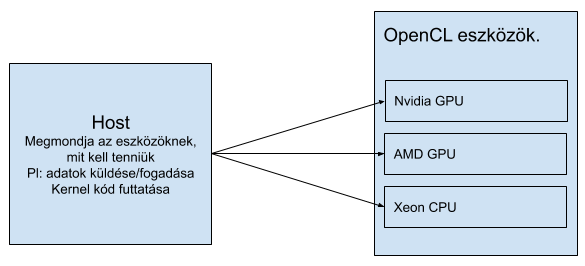
\includegraphics[width=\textwidth]{images/opencl.png}
\caption{\texttt{OpenCL}}
\label{fig:opencl}
\end{figure}

A következő esetekben a GPU-t érdemes használni:
\begin{itemize}
\item Gyors permutáció: Az eszközök gyorsabban mozgatáják a memóriát mint a Host.
\item Adat átváltás: Egyik formátumról másikra.
\item Numerikus gyorsítás: Az eszközök gyorsabban számolnak nagyobb adatdarabokkal mint a Host.
\end{itemize}
Jelen esetben a Host egy asztali számítógép.
Számítási eszközei: CPU, GPU, FPGA, DSP.
A számítási egységek: a magok száma
Elemek feldolgozása: ALU magonként.

\texttt{OpenCL} használata mellett szükségtelen gondolkozni azon, hogy pontosan mi is végzi el a számításokat. Ugyanis az \texttt{OpenCL} modelljének illeszkedése egy adott hardverhez, a gyártók feladata.

\begin{table}[h!]
\centering
\caption{CPU-k és GPU-k összehasonlítása}
\medskip
\label{tab:cpuvsgpu}
\begin{tabular}{|p{7cm}|p{7cm}|}
\hline
Alacsony számítási sűrűség & Magas számítási sűrűség \\
\hline
Komplex logikai vezérlő & Magas számítási és memória-hozzáférés \\
\hline
Nagy caches & Nincs nagyméretű gyorsítótár  \\
\hline
Optimalizált a soros műveletekre.
\begin{itemize}
	\item Kevesebb végrehajtási egység (ALU).
	\item Magas órajel sebesség.
\end{itemize} & Beépített párhuzamos műveletek.
\begin{itemize}
	\item Sok párhuzamos végrehajtási egység (ALU).
	\item A grafika a párhuzamosság legismertebb esete.
\end{itemize} \\
\hline
Keskeny adatvezeték <30 szakasz & Széles adatvezeték több száz szakasz \\
\hline
Alacsony késleltetési tolerancia & Magas áteresztőképesség, magas késleltetési tolerancia \\
\hline
Az újabb CPU-k több párhuzamosításra képesek & Újabb GPU-k
\begin{itemize}
	\item Jobb áramlást vezérlő logika
	\item Scatter/Gather Memory Access
	\item Már nem egyirányúak a pipeline-ok
\end{itemize} \\
\hline
\end{tabular}
\end{table}

\Section{Az OpenCL elemei}
\SubSection{Eszköz modell}

\begin{figure}[h!]
\centering
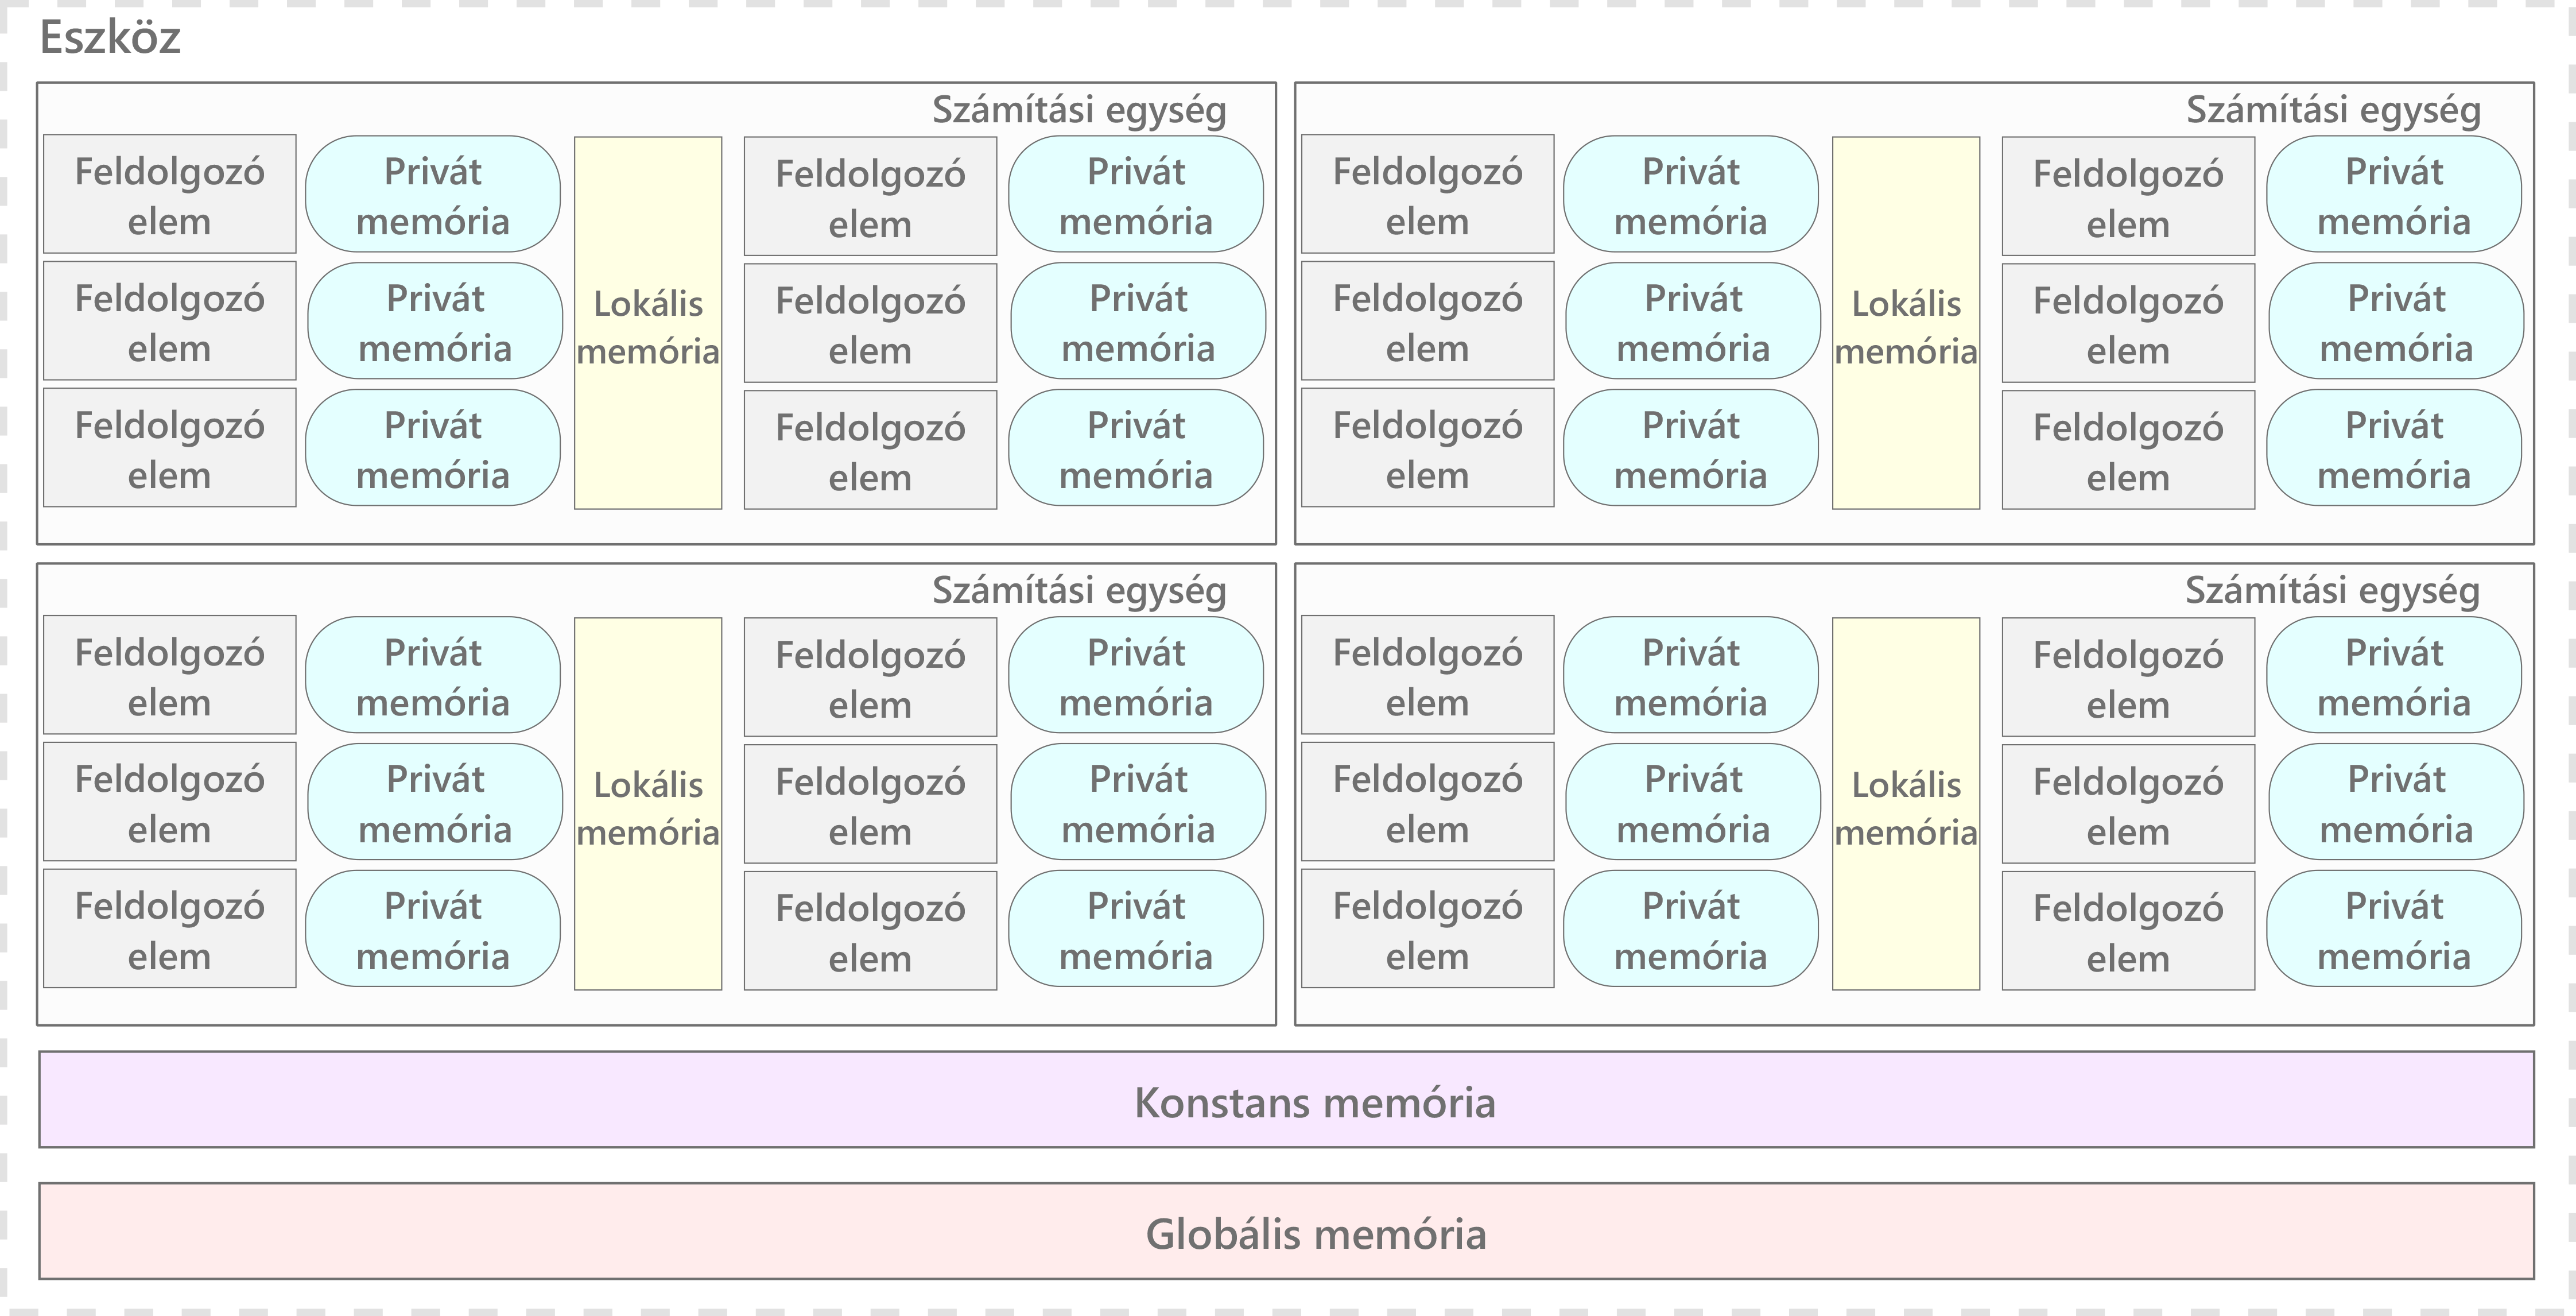
\includegraphics[width=\textwidth]{images/device.png}
\caption{\texttt{OpenCL} eszköz modell}
\label{fig:opencl}
\end{figure}

Négy féle memóriát különböztetünk meg:
\begin{itemize}
\item Globális memória: Minden eszközzel meg van osztva, de lassú. A kernel hívások között perzisztens. 
\item Konstans memória: Gyorsabb a globálisnál, szűrő paraméterek megadására használják.
\item Lokális memória: Minden számási egység számára privát, de megosztott a feldolgozó elemek között.
\item Privát memória: Gyorsabb a lokálisnál, minden feldolgozó elemnek van.
\end{itemize} 
A konstans, lokális és privát memóriába nem lehet adatokat menteni úgy, hogy más kernel használhassa majd azt.

\SubSection{Feldolgozási modell}

A Host -on \texttt{OpenCL} alkalmazások futnak amelyek a számítási eszközökhöz küldik a munkát.
\begin{itemize}
\item Munkaelem: A számítási eszköz alapvető egysége.
\item Kernel: A kód, ami fut a munkaegységen  (Alap C függvények)
\item Program: Kernelek és egyéb funkciók gyűjteménye
\item Kontextus: A környezet a munkaelemek végrehajtásához. (Eszközök, annak memóriái és parancssorai)
\item Parancssor: Sor melyet a Host arra használ, hogy a munkát (Kernelek, memória másolatok) az eszközbe küldje.
\end{itemize}

Ez egy keretrendszer, amely meghatározza, hogy a kernel hogyan hajtsa végre a probléma egyes pontjait. Vagy hogyan bontsa a feladatot munka elemekre.

Amire ehhez szükség van:
\begin{itemize}
\item Globális munkaméret. Ez általában egy bemeneti vektor teljes hossza.
\item Globális eltolás.
\item Munkacsoport méret.
\end{itemize}
Megfeleltetés:
\begin{itemize}
\item Munkaelem - számítási elem: Minden munkaelemet egy számítási elem hajt végre.
\item Munkacsoport - számítási egység: Minden munkacsoportot egy számítási egység hajt végre. A munkacsoport munkaelemek, a számítási egység pedig számítási elemek csoportja.
\item Kernel végrehajtási példány - Számítási eszköz. Munkacsoportok összessége illetve számítási elemek összessége. 
\end{itemize}

\SubSection{Munkacsoportok}

Ideális esetben végtelen számú feldolgozási elemmel rendelkezik az eszköz, Minden ilyen elem az adatok egy részét kezeli anélkül, hogy szükségük lenne kommunikációra. De ez a gyakorlatban nem szokott ilyen egyszerű lenni, ezért a munkát fel kell osztani.
\begin{itemize}
\item A teljes munkát fel kell osztani kisebb darabokra.
\item Minden darab egy munkacsoporthoz tartozik.
\item A munkacsoportokat ütemezéssel kell végrehajtani a számítási egységeken.
\item Minden csoport rendelkezik egy megosztott memóriával, ami olyan mint a lokális memória a számítási-egységeknél
\end{itemize}
A folytatáshoz a munkacsoportokat ütemezni kell a végrehajtási egységeken, és a munkaelemeket számítási egységen belül végrehajtani.
Minden munkaelem társulni fog egy számítási egységhez, ha van elegendő. Ezt a folyamatot az \texttt{OpenCL} végzi, csak meg kell adni a globális munkaméretet és munkacsoport méretet. A kernelt indító függvény a  munkacsoportok számát kiszámolja. Ha nincs elég számítási egység, akkor a munkacsoportok sorban hajtódnak végre a meglévő egységeken.

\SubSection{\texttt{OpenCL} program általános felépítése}
\begin{itemize}
\item Létre kell hozni egy szöveg típusú változót, ami tartalmazza a kernel kódot.
\item Definiálni kell az eszközt, kontextust és parancssort.
\item Definiálni kell a szükséges memória puffereket.
\item Az adatokat be kell másolni a pufferekbe.
\item Létre kell hozni a programot a szövegből.
\item Fel kell építeni a programot.
\item Létre kell hozni a kernelt és be kell állítani a paramétereit.
\item Futtatni kell a kernel kódot.
\item Ki kell olvasni a memóriaobjektumokban található választ a Host-on.

\end{itemize}


\SubSection{Az \texttt{OpenCL} telepítése}

A megfelelő működéshez az első lépést már a rendszer telepítésénél megtettem amikor a non-free avagy az nvidia eredeti drivernének a telepítését választottam.
ezen kívül a következő csomagokra volt szükség: 

\begin{python}
$ sudo pacman -S opencl-headers
$ sudo pacman -S opencl-nvidia
$ sudo pacman -S cuda
$ sudo pacman -S ocl-icd
\end{python}


\Chapter{Megvalósítás}

Az alap ötlet egyszerű. A MySQL szerverről lekérjük a tábla tartalmát, amit be másolunk az \texttt{OpenCL} pufferébe, majd a kernelkód futtatása után az eredményt tartalmazó részeket kiolvassuk. De felvetődik pár problémás rész. Hogyan tároljuk a tábla tartalmát? Mekkora legyen a Globális munkaméret és a munkacsoport méret? Milyen formában állítsuk elő az eredményt, és hogyan olvassuk azt ki?


\Section{Adatok előkészítése}

\SubSection{Táblák tömbbé alakítása}
Ahhoz, hogy \texttt{OpenCL} el kezelni tudjuk az adatokat először szükség lesz egy struktúrára ami reprezentálja az adatbázis tábla felépítését. Az az a struktúra adattagjainak típusa egyezzen meg a táblázat oszlopainak típusával. Ezek után ebből létre kell hoznunk egy tömböt melynek hossza legalább annyi, mint a tábla sorainak száma.

\begin{figure}[h!]
\centering
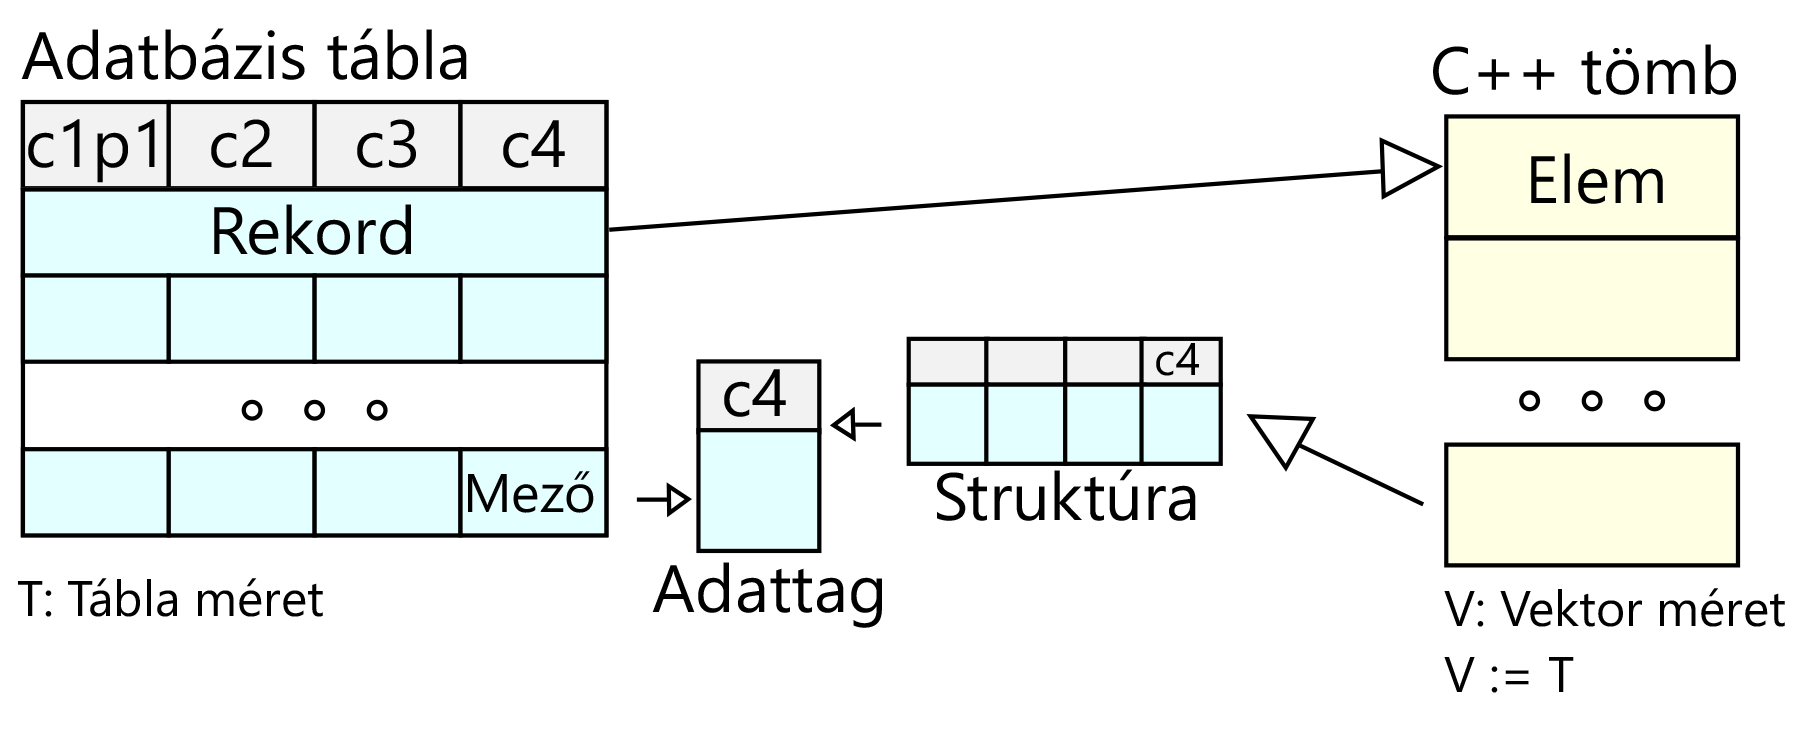
\includegraphics[width=11cm]{images/data/structure.png}
\caption{Adatbázistábla átalakítása tömbbé}
\label{fig:opencl}
\end{figure}

\begin{itemize}
\item A struktúra megfelel a tábla felépítésének.
\item A tömb egy eleme, egy ilyen struktúra.
\item A tömb egy eleme megfelel a tábla egy rekordjának azaz sorának.
\item Egy elem adattagjai megfelelnek az adatbázis egyazon rekordjához tartozó mezőknek.
\end{itemize}

\newpage
\SubSection{A táblákat beolvasó függvény.}

A fix sorszámmal rendelkező adatbázis táblák kezelése egy nagyon speciális eset lenne, ezért a programot úgy kell megírni, hogy igazodni tudjon a különböző táblaméretekhez.

Mivel a tábla méret előre nem ismert ezért a tömböket a \texttt{malloc} függvénnyel lehet lefoglalni. De mivel a lekérdezést külön függvény végzi, és a méretet sem tudjuk előre, ezért a következő megoldást alkalmazom:
Első lépésben létrehozok egy pointert ami később a táblára fog mutatni, most még \texttt{NULL} értékű, és ehhez egy változót ami a méretet tárolja. Az adatokat lekérő függvénynek átadom ezeket, és miután a \texttt{Connector} elvégezte a lekérdezést beállítom a méret változó értékét illetve a tábla memória területét csak ekkor foglalom le, és állítom rá a pointert. Ez úgy lehetséges, hogy a függvénynek egy pointerre mutató pointert adok át, ezáltal kettős indirektség jön létre.

\begin{cpp}
Table1Type *t1 = NULL;
int t1_size;
load_database(&t1, &t1_size);
	
res = pstmt->executeQuery();
\end{cpp}
\begin{figure}[h!]
\centering
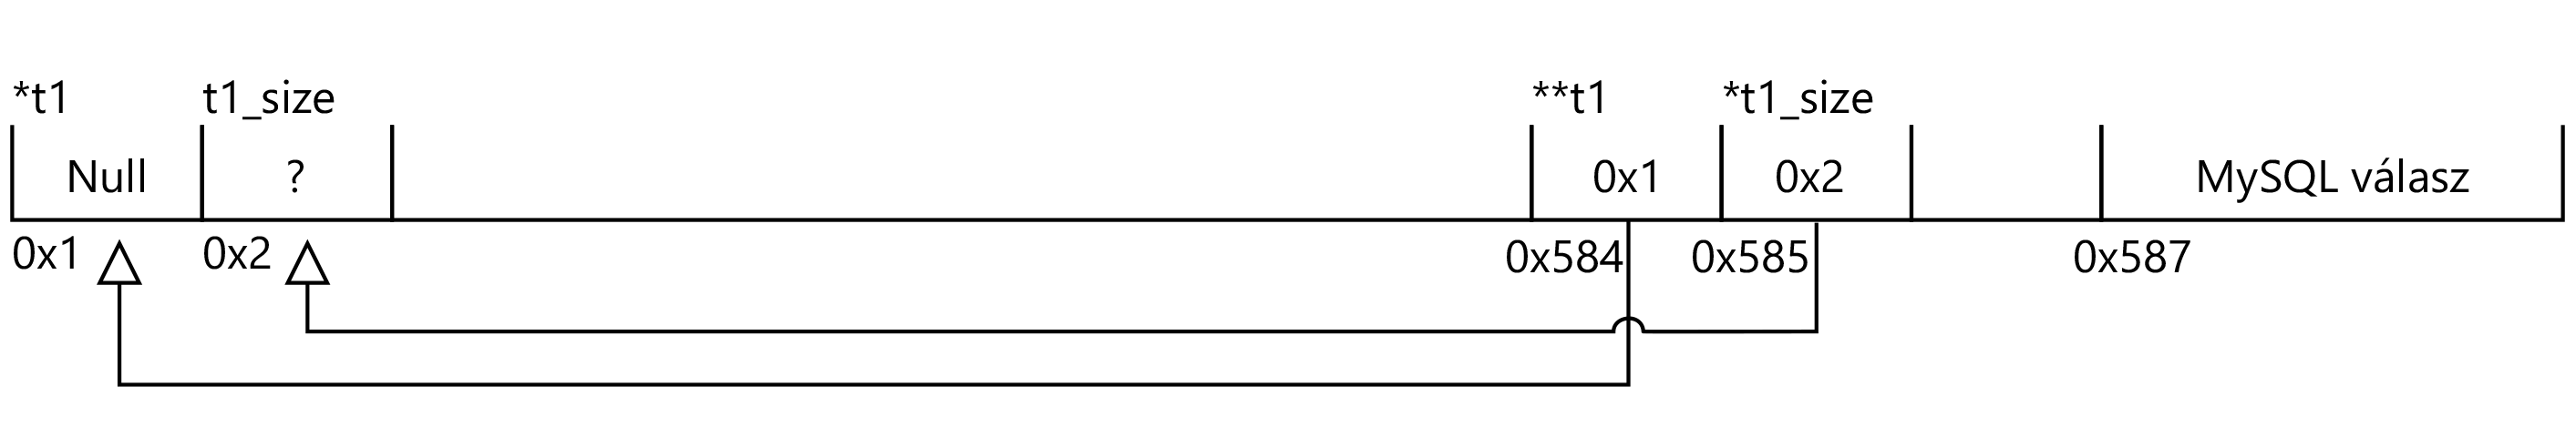
\includegraphics[width=\textwidth]{images/implementation/pointer_01.png}
\caption{Pointerek a létrehozáskor}
\label{fig:opencl}
\end{figure}
\begin{cpp}
int i = 0;
*T1_size = res->rowsCount();
*T1 = (Table1Type*) malloc(sizeof(Table1Type) * *T1_size);

while (res->next()) {
  T1[0][i].c1p1 = res->getInt("c1p1"); T1[0][i].c2 = res->getInt("c2");
  T1[0][i].c3 = res->getInt("c3"); T1[0][i].c4 = res->getInt("c4");
  i++;
}
\end{cpp}
\begin{figure}[h!]
\centering
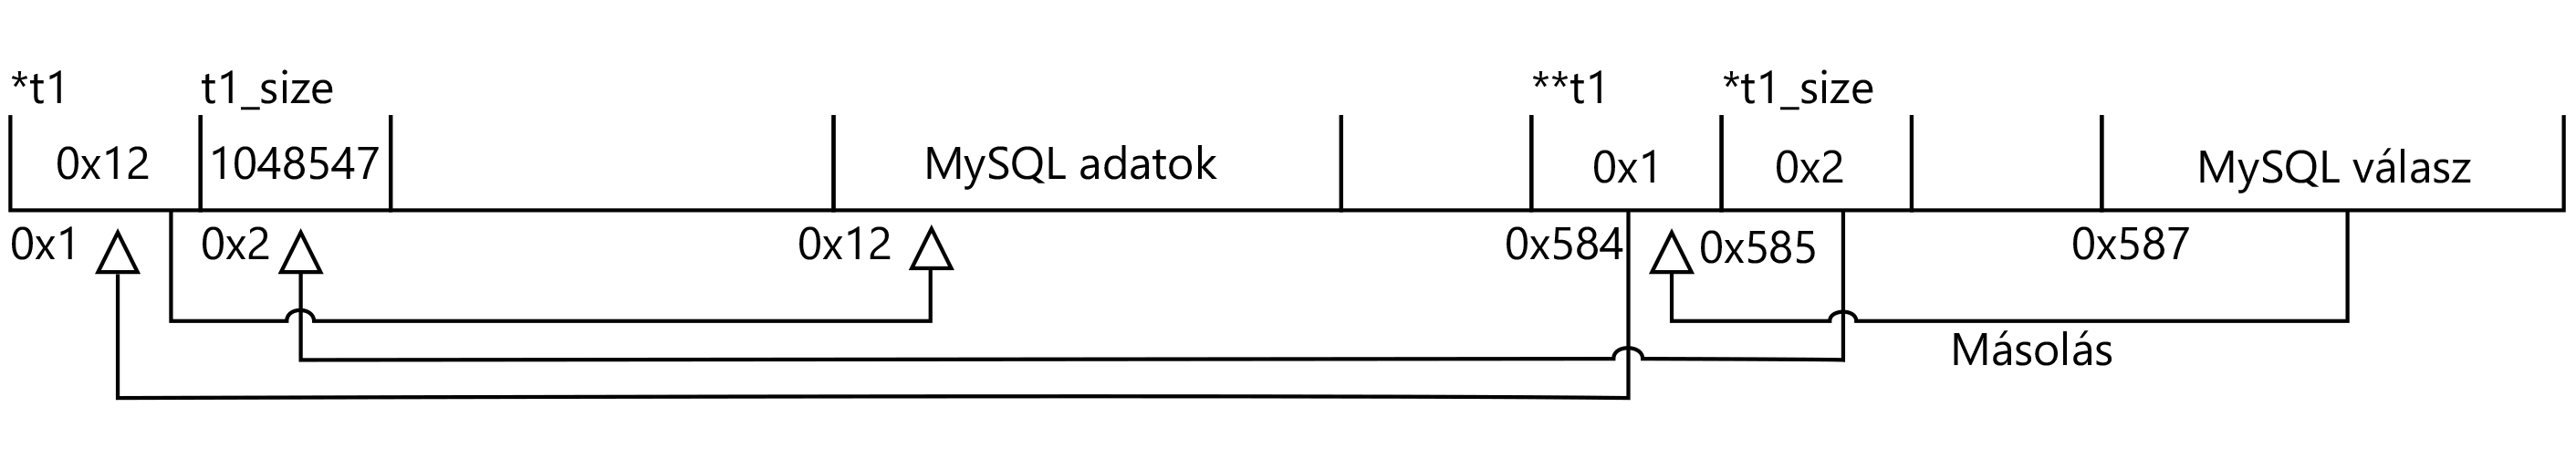
\includegraphics[width=\textwidth]{images/implementation/pointer_02.png}
\caption{Pointerek teljes működése}
\label{fig:opencl}
\end{figure}

\Section{Globális és lokális méret meghatározása}
Ennél a pontnál oda kell figyelni pár alapvető dologra:
\begin{itemize}
\item A lokális méret legfeljebb 1024 lehet.
\item A globális méretnek a lokális többszörösének kell lennie.
\item A túl sok vagy túl kevés munkacsoport használata esetén a párhuzamosság sérül.
\item A munkacsoportok és csoporton belül a munkaelemek feldolgozása párhuzamos.
\item Munkacsoportok között nem lehetséges szinkronizáció, csak munka elemek között, amennyiben azok egy munkacsoportba tartoznak.
\item Nem használható kölcsönös kizárás, a szemafor végtelen ciklushoz vezet.
\end{itemize}

\SubSection{Működési elv}

Egyszerű esetben a bementi elemszámot megadhatjuk mint globális méret, ez a gyakorlatban meghatározza, hogy hányszor fog lefutni a kernel függvény. A $get\_global\_id(0)$ meghívásával megkapjuk az aktuális azonosítót, ez 0 -tól globális méret -1 ig terjed. Innentől tekinthetünk a teljes kódra úgy, mintha egy párhuzamos futó \texttt{for} ciklusban lenne.

Ezen kívül meg kell adnunk a lokális méretet, ami az elemek száma egy munkacsoporton belül. A kernel futása közben ezt is megkaphatjuk a $get\_local\_id(0)$ használatával, csak úgy mint a munkacsoport azonosítót vagy az említett paraméterek méretét.

A végeredményt tartalmazó kimeneti tömb hossza egyezik a globális mérettel, így nem ütközhetünk bele abba a hibába, hogy két számítási elem ugyan oda próbáljon írni. Amennyiben például az 545. elem megfelel, akkor az indexe és egyéb hozzá tartozó értékek az 545. helyen lesznek a kimeneti tömbben.

\begin{figure}[h!]
\centering
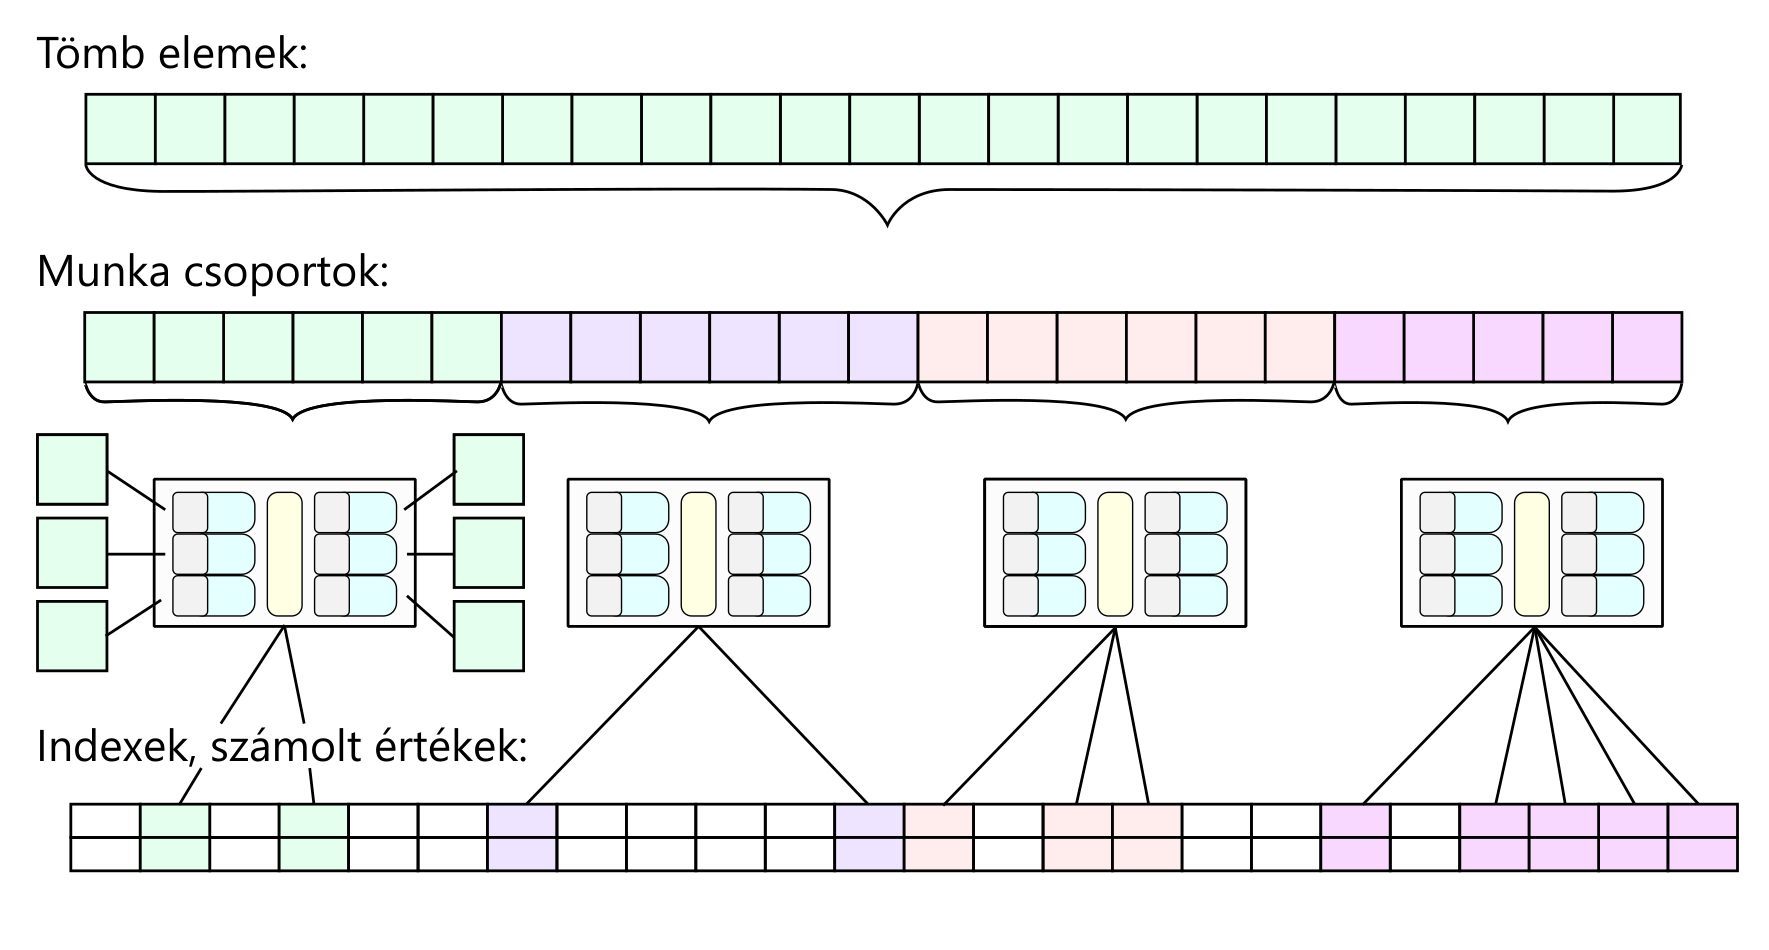
\includegraphics[width=\textwidth]{images/workgroups_black.png}
\caption{Munkacsoportokra bontás}
\label{fig:opencl}
\end{figure}

\newpage

\SubSection{Globális méret meghatározása}
Tegyünk fel, hogy kaptunk egy 1048547 sorból álló táblázatot. Ekkor több probléma is előkerül. Egyrészt olyan lokális méretet kell választani ami ennek a számnak az osztója. Másfelől nem szeretnénk végignézni az ugyan ilyen hosszú kimeneti tömböt az eredmények helyét keresve.

A következő módon oldottam meg a problémát: Állítsuk a globális méretet például 1024 -re, ehhez határozzunk meg egy intervallum méretet a sorok száma és globális méret hányadosának felső egész része ként. Ez jelen esetben szintén 1024 lesz. Viszont így át kell adnunk a kernelnek a tábla méretét, ami felső határként ügyel arra, hogy ne lépjük túl a tömböt méretét.

A módosításnak az lesz a következménye, hogy egy munkaelem nem csak a tömb egy elemén fog dolgozni hanem egy intervallumán. Ezzel létrehoztunk olyan részeket a tömbben amiknek a feldolgozása biztosan soros lesz. Ennek köszönhetően már tudunk használni számlálókat, nincs szükség kölcsönös kizárásra. A számlálókat tartalmazó tömb mérete megegyezik a globális mérettel.

Ezekhez a paraméterekhez még tetszőlegesen meg kell határozni a lokális méretet, aminek csak a teljesítményre van hatása.


$$ global\_size = 1024 $$
$$interval\_size =  \left\lfloor \frac{table\_size }{globalsize\_size} \right\rfloor  +1  $$


\SubSection{A kernelkód működése}

A kernel meghatározza saját globális azonosítóját és ebből illetve a kapott intervallum méretből kiszámítja, honnan kezdőik az ő része a be-, és kimeneti tömbön. Ezután elkezdi az intervallumnyi elem vizsgálatát ügyelve arra, hogy a tábla méretet ne lépje túl. Amennyiben egy elem megfelel a szűrési paramétereknek annak indexét és egyéb lekérdezés függő kiszámolt értékeket a kimeneti tömbbe másol, majd növeli saját számlálóját. Ez a számláló határozza meg, hogy a kimeneti szakaszon a következő elem hányadik helyre kerüljön.
\begin{figure}[h!]
\centering
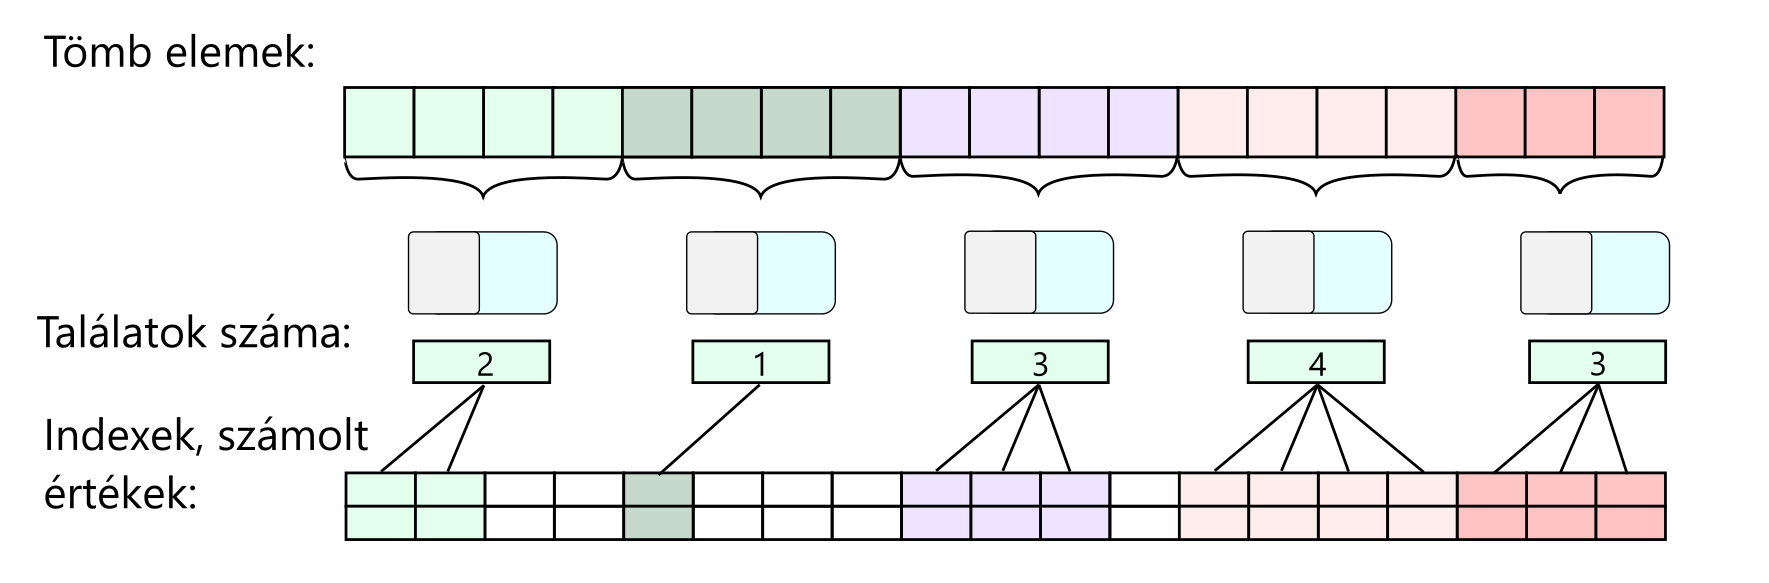
\includegraphics[width=\textwidth]{images/itemgroup_black.png}
\caption{Intervallumok feldolgozása}
\label{fig:opencl}
\end{figure}
Itt már nem munkacsoportonként, hanem feldolgozó elemenként látjuk a folyamatot.

\newpage
\Section{Eredmény kiolvasása}
A kernelkód működéséből látjuk, hogy több módszert is tudunk alkalmazni az elemek kiolvasására. A találatok számát tartalmazó tömböt biztosan ki kell másolnunk, de kimenetre vonatkozóan nézzük meg az alábbi lehetőségeket.
\SubSection{Az elemek kiolvasása egyben}

Dönthetünk úgy, hogy kimásoljuk a teljes kimenetet:
\begin{python}
clStatus = clEnqueueReadBuffer(command_queue, TableResult_clmem, 
	CL_TRUE, 0, table_size * sizeof(TableResultType), result, 
	0, NULL, NULL);
\end{python}
Ekkor ennek olvasása a következőképpen zajlik:
\begin{python}
for(i=0; i< global_size; i++)
{
  offset = i*interval_size;
  
  for(j=0; j<result_counter[i]; j++)
  	cout << t1[ result[ offset + j ].index ].c1p1 << endl;
}
\end{python}
Végig kell menni a számlálón aminek hossza \texttt{global size}, majd az \texttt{ i * interval size} eltolást használva annyi elemet kell sorban kiolvasni az adott részről, amekkora érték a hozzá tartozó számlálóban található. Ezzel végig lépkedve és ugrálva a kimeneten ki tudjuk olvasni az indexeket illetve kiszámított értékeket.

\SubSection{Az elemek kiolvasása szakaszosan}
A másik módszer, hogy csak az információkat tartalmazó részeket olvassuk a pufferekből. Ez hasonló módon zajlik, mint előző esetben az eredmények kiírása.

\begin{python}
int count = 0;
for(int i=0; i< global_size; i++)
{
if(result_counter[i] < 1 ) continue; 
clStatus = clEnqueueReadBuffer(command_queue, TableResult_clmem, CL_TRUE, 
	i*interval_size * sizeof(TableResultType),
	result_counter[i]* sizeof(TableResultType), 
	&result[count], 0, NULL, NULL);
	count+=result_counter[i];
}
\end{python}

Kiolvasásnál megadjuk az eltolást amit az előző módon számolunk annyi különbséggel, hogy megadjuk egy elem memória méretét:
$$i * interval\_size * sizeof(TableResultType)$$ezután megadjuk, hogy az eltolástól kezdve mekkora memória méretet szeretnénk kiolvasni: $$result\_counter[i] * sizeof(TableResultType)$$Ezen kívül a másolás cél memóriacímét mindig eltoljuk, az eddigi találatok számával: $$\&result[count].$$
Ha memóriát is szeretnénk spórolni, megtehetjük azt is, hogy először összeadjuk a találatokat és az alapján foglaljuk le a memóriaterületet a kiolvasáshoz.
\begin{figure}[h!]
\centering
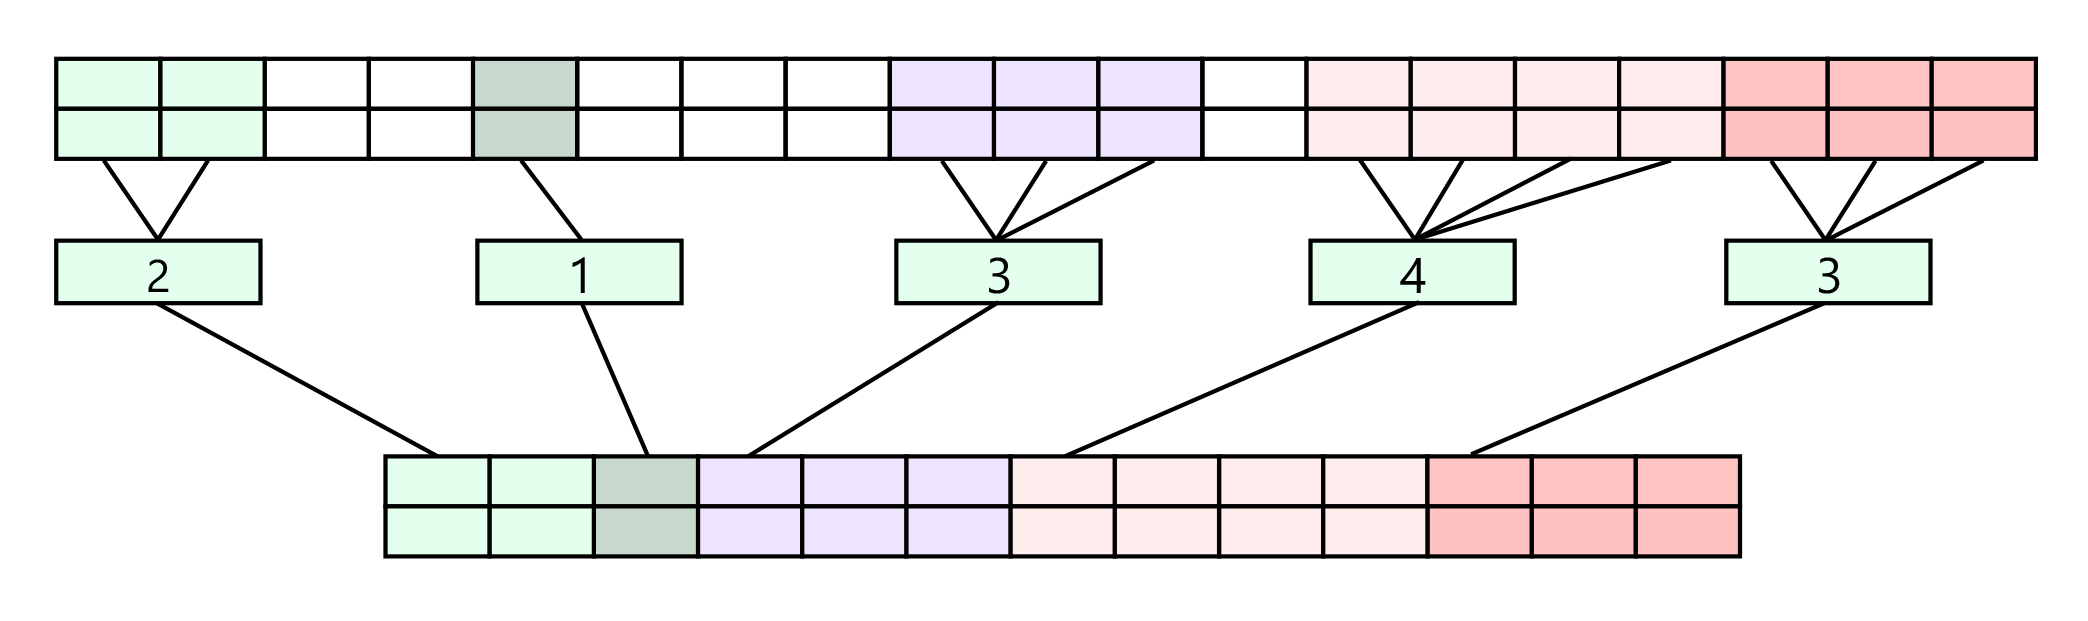
\includegraphics[width=\textwidth]{images/copy_02.png}
\caption{Munkacsoportokra bontás}
\label{fig:opencl}
\end{figure}
\newpage
\Section{Összetett lekérdezés}

Az előzőekben taglalt elméleti részek egy táblás lekérdezésekre vonatkozóan próbálták szemléltetni, milyen logika alapján lehet egy \texttt{SQL} lekérdezést \texttt{GPU} -n párhuzamosítva végrehajtani.
Most gondoljuk át, miképpen lehetne megoldani kettő vagy több tábla összekapcsolását. Első lépésben a lekérdezést egy-egy táblára vonatkozó részekre. Ezzel két tábla kapcsolása esetén létrejöhet két különálló kernel amelyek például a szűréseket végzik a táblákon. Ennél a lépélnél két dolgot is szükséges kiemelni. Egyrészt ezeknek a kerneleknek az előállított eredményét nem kell kiolvasni a pufferekből, ugyanis ez a globális memóriában van, így átadható másik kernel számára is. Másrészt pedig ezek a kernelek ha van kapacitás, akkor futhatnak párhuzamosan is, ezt úgy lehet elérni, hogy külön parancssort hozunk létre számukra.

Miután minden nem összekapcsolást végző kernel befejezte a munkát, adjuk át a szükséges paramétereket a befejező kernelnek. A paraméter lista elég hosszú lesz, ennek az az oka, hogy az eredmények kiolvasása elő észében taglalt módon kell végig menni a szűrt táblákon. 

Ennek a kernelnek a globális mérete egyezzen meg a lekérdezésben szereplő legnagyobb tábla globális méretével és ez a tábla szerepeljen a külső ciklusban. Az eredményeket változatlan módokon lehet majd kiolvasni a főprogramba.

\begin{figure}[h!]
\centering
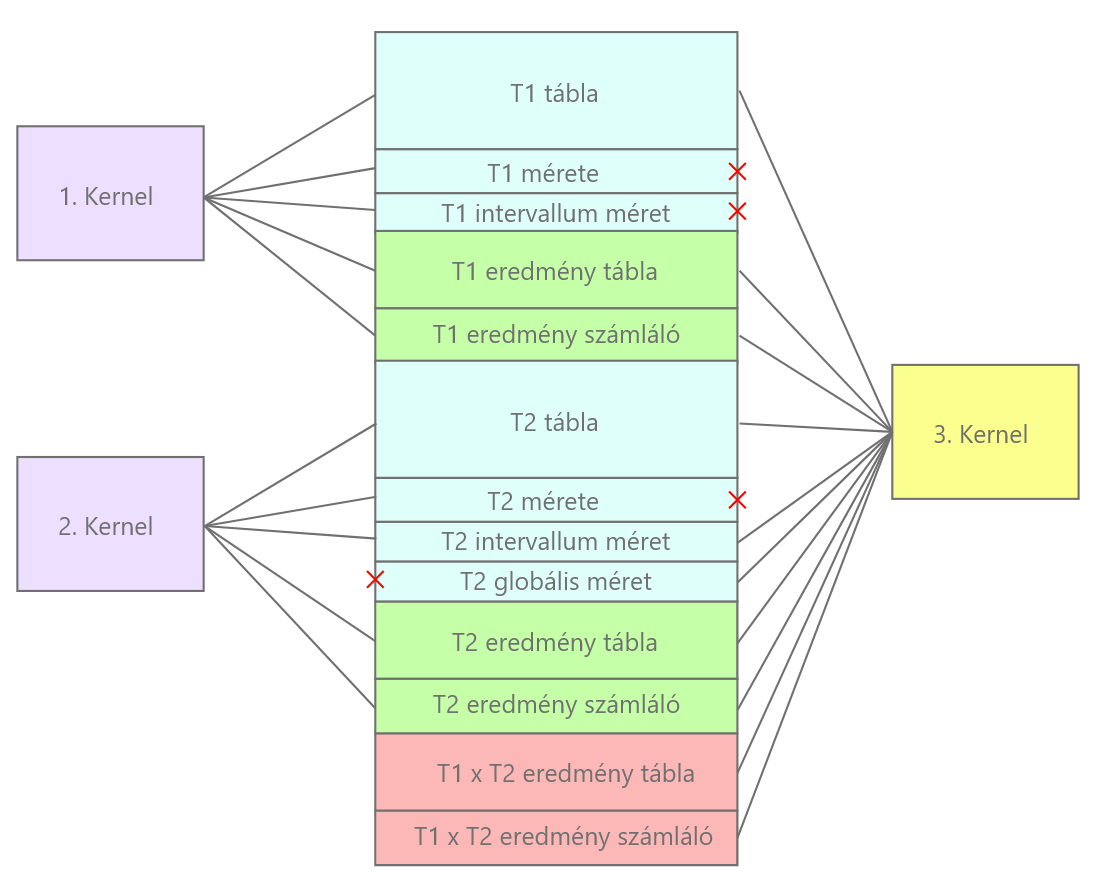
\includegraphics[width=12cm]{images/join_kernels.png}
\caption{Kernelek munkaterületei }
\label{fig:opencl}
\end{figure}

Az 1. és 2. kernel az előzőekben taglalt módon előállítja saját eredményeit (zöld rész). 
A 3. kernel megkapja a két táblát, a 2. tábla méretét és az előző két kernel által előállított eredményeket.
Az első eredmény kiolvasási módszer alkalmazásával és a kulcsok figyelésével a két táblát összekapcsoljuk és előállítjuk az eredményt.
A táblák méretére nincsen szükség, ugyanis az eredmény biztosan nem tartalmaz olyan indexet ami kívül esne az eredeti táblákon. A második táblánál viszont szükség van a globális méretre és az intervallum méretre a kiolvasáshoz.


